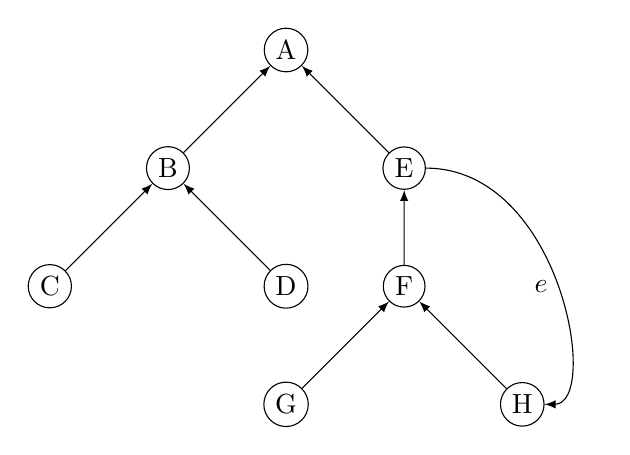
\begin{tikzpicture}[>=latex,level/.style={sibling distance=3cm}]
	\node[circle,draw,inner sep=2] {A}
		child[<-] {node[circle,draw,inner sep=2] {B}
			child {node[circle,draw,inner sep=2] {C}}
			child {node[circle,draw,inner sep=2] {D}}
		}
		child[<-] {node[circle,draw,inner sep=2] (E) {E}
			child {node[circle,draw,inner sep=2] {F}
				child {node[circle,draw,inner sep=2] {G}}
				child {node[circle,draw,inner sep=2] (H) {H}}
			}
		};
	\draw[->] (E) .. controls +(right:2) and +(right:1) .. node[left] {$e$}(H);
\end{tikzpicture}

